\section{Preface}
\label{ch:introduction:preface}
Sound systems are used world wide to fill rooms with enjoyable audio content. 
Problems arise however when multiple people in the same room want to enjoy different audio content at the same time.

For example, one person may want to enjoy a movie on the television, while another may want to listen to their music.
If they are in the same room, their desires clash: neither person can fully enjoy their chosen activity without disturbing
the other.
In short, the interference of multiple source of audio leads to a situation where both individual experiences are diminished.

In recent years, attempts have been made to solve this problem by controlling the spatial reproduction of sound in such
a way that different areas in a room have distinct content.

One class of algorithms that attempt to do so are sound zone algorithms~\cite{betlehem2015personal}.
Sound zone algorithms partition the space of the room into multiple so-called sound zones.
Each sound zone is assigned different audio content.
The sound zone algorithms decides how to use the loudspeakers of the sound system to reproduce said audio content in every zone.
Using the principals of constructive and destructive interference, this is done in such that there is minimal interference between zones.
That is to say: the audio content of each zone is not audible in the others.

In the previously listed example, one zone would contain the audio of a movie and another zone would contain music.
An image depicting the situation is given in \autoref{fig:introduction:motivation:concept}.
The sound zone algorithm determines how to best use the sound system to reproduce these two zones.
In the ideal case, both people can now enjoy the full potential of their audio content, without bothering one another.

\begin{figure}[]
    \centering
    \scalebox{1.0}{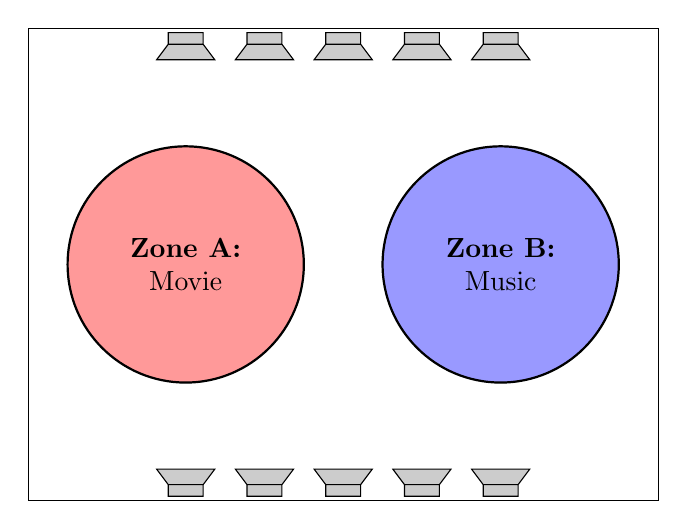
\begin{tikzpicture}
    \tikzset{
      Speaker/.pic={
        \filldraw[fill=gray!40,pic actions] 
        (-15pt,0) -- 
          coordinate[midway] (-front) 
        (15pt,0) -- 
        ++([shift={(-6pt,8pt)}]0pt,0pt) coordinate (aux1) -- 
        ++(-18pt,0) coordinate (aux2) 
        -- cycle 
        (aux1) -- ++(0,6pt) -- coordinate[midway] (-back) ++(-18pt,0) -- (aux2);
      }
    }

    \draw [draw=black] (0,0) rectangle (8,6);

    % Speakers on the top wall
    \pic[scale=0.7] at (2, 5.6) {Speaker};
    \pic[scale=0.7] at (3, 5.6) {Speaker};
    \pic[scale=0.7] at (4, 5.6) {Speaker};
    \pic[scale=0.7] at (5, 5.6) {Speaker};
    \pic[scale=0.7] at (6, 5.6) {Speaker};

    % Speakers on the bottom wall
    \pic[rotate=180, scale=0.7] at (2, 0.4) {Speaker};
    \pic[rotate=180, scale=0.7] at (3, 0.4) {Speaker};
    \pic[rotate=180, scale=0.7] at (4, 0.4) {Speaker};
    \pic[rotate=180, scale=0.7] at (5, 0.4) {Speaker};
    \pic[rotate=180, scale=0.7] at (6, 0.4) {Speaker};

    \draw[opacity=0.4, fill=blue] (6,3) circle[radius=1.5];
    \draw[thick] (6,3) circle (1.5) node[align=center] {\textbf{Zone B:}\\Music};
    \draw[opacity=0.4, fill=red]  (2,3) circle[radius=1.5];
    \draw[thick] (2,3) circle (1.5) node[align=center] {\textbf{Zone A:}\\Movie};
\end{tikzpicture}
}
    \caption{A room containing a sound system consisting of an array of loudspeakers and two zones.
                The goal of the sound zone algorithm is to control the sound system in such a way that the red zone
                contains the audio of a movie, and the blue zone contains the music.}
    \label{fig:introduction:motivation:concept}
\end{figure}

In practice however, the sound zone algorithm will not always do a perfect job.
The performance of algorithms depends on the environment and the available sound system.
Depending on the situation, the interference between zones can typically only be reduced by so much.
As such, audio content of one zone is often still audible in other zones.

Improving sound zone algorithms is thus still an active topic of research.
One recent approach is to include a model of the human auditory system, which models how sound is perceived by humans.
Typically, sound zone algorithms use sound pressure, which is a physical quantity characterizing the sound.
Sound pressure does not always accurately describe what is important for the perception of sound.
As such, including a perceptual model may allow the algorithm to focus on the parts of the audio content
that matter perceptually.

Early results show that the perceptual sound zone approach is promising.
Recent work by Donley et al. explored including the absolute threshold of hearing, which models the lowest sound pressure
humans can hear, into sound zone algorithms.
This pursuit found an increased quality of the reproduced audio in the zones~\cite{donley2015multizone}.
Other work by Lee et al. showed that including a perceptually-motivated weighting in the sound zone algorithm outperforms 
traditional algorithms~\cite{lee2019towards,lee2020signal}.

This work seeks to further explore this perceptual approach by proposing a novel perceptual sound zone algorithm and exploring
the benefits of including perceptual information.
